\documentclass[FM,BP]{tulthesis}  % Bakalářská práce fakulty mechatroniky
\usepackage[czech]{babel}  % Česká šablona dokumentu
\usepackage[utf8]{inputenc}  % Česká diakritika
\usepackage{graphicx}  % Tvorbě tabulek
\usepackage{float}  % Ukotvení věcí na svém místě (obrázky, tabulky, grafy, ...)
\usepackage{hyperref}  % Klikací odkazy v obsahu a referencích

\TULtitle{Koncept nízkonákladového sledovacího zařízení pro osobní automobily}{The concept of a low cost tracking device for personal cars}
\TULprogramme{B2646}{Informační technologie}{Information Technology}
\TULbranch{1802R007}{Informační technologie}{Information Technology}
\TULauthor{Tomáš Moravec}
\TULsupervisor{Ing. Lenka Kosková Třísková}
\TULyear{2016}

\begin{document}
\ThesisStart{male}

\begin{acknowledgement}
Děkuji vedoucí práce paní Ing. Lence Koskové Třískové za odborné vedení a poskytnuté informace při zpracování závěrečné bakalářské práce. Mé poděkování patří též Tomáši Stránskému za sdílení praktických zkušeností s použitými komponenty.
\end{acknowledgement}

\begin{abstractCZ}
Práce se zabývá problematikou sledovacích zařízení pro osobní automobily. V úvodu je definován pojem sledovacího zařízení a požadovaných vlastností. Následuje rešerše aktuální situace na trhu a srovnání užitých konceptů pro realizaci sledovacích zařízení. Na základě rešerše je navržen koncept sledovacího zařízení pro osobní automobily s cílem vytvořit levné a spolehlivé zařízení pro střední a nižší třídu vozů. Výstupem práce je prototyp cílového zařízení, který demonstruje zvolené hardwarové i softwarové řešení.
\end{abstractCZ}

\vspace{2cm}

\begin{abstractEN}
Thesis deals with tracking devices for cars. The introduction defines the concept of surveillance equipment and required attributes. Following a research of the current market situation and comparison of the concepts used for implementing surveillance equipment. Based on the research is designed concept of tracking devices for cars in order to create a cheap and reliable device for middle and lower class cars. The outcome of this work is the prototype of the target device, which demonstrates the chosen hardware and software solution.
\end{abstractEN}

\tableofcontents
\clearpage

\begin{abbrList}
\textbf{SMS} & Short message service, služba pro přenost krátkých textových zpráv\\
\textbf{GPS} & Global Positioning System, družicový polohovací systém\\
\textbf{GSM} & Groupe Spécial Mobile, globální systém pro mobilní komunikaci\\
\textbf{GPRS} & General Packet Radio Service, služba pro přenos dat v mobilní síti\\
\textbf{GLONASS} & Globalnaja navigacionnaja sputnikovaja sistěma, globální navigační satelitní systém\\
\end{abbrList}

% Úvod

\chapter{Úvod}
Podnětem vytvoření této práce mi byl můj vlastní zájem o sledovací zařízení do automobilu, kdy jsem pátral po levném, kvalitním, jednoduše ovladatelném zařízení, které naplní moje požadavky. Nejdříve jsem prohledal české portofilo a když jsem zjistil že zařízení, která splňují moje požadavky jsou cenově odhodnoceny kolem 8 000 Kč, rozhodl jsem se pro nákup u Číny. První zařízení za 400 Kč, které i přes popis o funkčnosti po celém světě, nebylo schopné fungování v České republice, mapové podklady na Evropu nebyly připraveny a odpovědi na SMS chodili v čínském jazyce, stejně tak manuál byl čínsky. Další pokus nastal se zařízením za 600 Kč, kdy zařízení odpovídalo na SMS nečitelnou změtí písmen a číslic, mapové podklady byly tentokrát přes Google, ale přesnost byla na stovky metrů a většinou se trefilo o několik ulic vedle. Řekl jsem si musí to jít přeci udělat lépe.

% Sledovací zařízení

\chapter{Sledovací zařízení}
Sledovací zařízení je přístroj, udávající svou vlastní polohu na planetě zemi, pomocí zeměpisné šířky a délky. Poloha se určuje vzhledem k systému družic GPS, které obíhají rovnoměrně rozprostřeny na oběžné dráze země. Typicky slouží ke sledování osob, vozidel, či nákladu a jeho využití najdou jak běžní domácí uživatelé a bezpečnostní agentury, usilující o bezpečnost vozidel, podniky monitorující pohyb svého vozového parku (Fleet management), nebo velké logistické společnosti, sledující pohyby zásilek nebo kontejnerů. Přesnost polohy je pro uživatelský sektor desítky metrů, zatím co autorizovaní uživatelé (americká armáda a vybrané spojenecké armády) mají k dispozici přesnost v jednotkách metrů. Vyšší přesnosti se dosahuje mnoha způsoby, jako například mobilní sítě, jiné navigační systémy, matematické výpočty. Za ideálních podmínek lze přesnost zvýšit i na jednotky centimetrů. Přesnost vertikální je zpravidla 2x až 3x tak horší než zmiňovaná horizontální.

\section{Historie}
Polohovací systém GPS je vojenský globální družicový systém, provozovaný Ministerstvem obrany Spojených států amerických. Projekt navazuje na předchozí NAVSTAR GPS a od roku 1978 bylo do dnešního dne vypuštěno celkem 32 družic. Družice nebyly vpouštěny pouze za účelem určování polohy pro navádění raket a dalších zařízení, ale také aby detekovali vypuštění balistických raket a výbuchy jaderných bomb. Všechny satelity byly také vybaveny přesnými atomovými hodinami, které dnes dodávají přesný čas po celé zemi. Původně vojenský projekt se stal dostupným i pro neautorizované uživatele z finančních důvodů, aby nemusel být zrušen. V roce 1990 během války v Zálivu byla dočasně deaktivována dostupnost pro neautorizované uživatele a zapojena byla opět v roce 1991.

\section{Přítomnost}
Satelitní systém GPS se stal synonymem pro sledovací zařízení a určování polohy a je celosvětově využíván ve všech lidských odvětvých. Nicméně dnes není jediným projektem poskytujícím zěměpisnou polohu. Od roku 2011 je k dispozici ruský armádní polohový systém GLONASS, který se vyznačuje stejnou přesností jako systém GPS. Pomalu ale jistě se dostává do povědomí a většina nejnovějších mobilních zařízení umí komunikovat nejenom s GPS, ale také s GLONASS, získáváním dat z více než jednoho systému satelitů, poskytuje výrazné zvýšení přesnost polohy. Posledním, zatím nedokončeným je evropský navigační systém Galileo, který má od roku 2012 nové sídlo v Praze, měl být částečně funkční v roce 2015 (18 satelitů) a plně dokončen roku 2019/20 (30 satelitů). Bohužel v roce 2014 přišel systém o dvě nové družice, které měl vynést ruský nosič, bohužel mu selhal poslední stupeň rakety a obě byly vyneseny na špatnou oběžnou dráhu, na které jsou dodnes. Později roku 2014 byla vynesena první družice na správnou oběžnou dráhu, poté byl projekt pozastaven do té doby, než se podaří vyřešit, jak do systému zapojit družice na špatné oběžné dráze.

% Požadované vlastnosti

\section{Požadované vlastnosti}
V honu za kvalitním, ale levným sledovacím zařízením, je nutné nalézt kompromis mezi nízkou cenou a pohodlím zákazníka. Abych tohoto docílil, budu se snažit vyzdvihnout vlastnosti, které neovlivní cenu, ale výrazně posílí funkčnost a tím i konkurence schopnost zařízení. Následující vlastnosti pro mne budou hrát důležitou roli při výběru hardwarových součástek, stejně tak mi pomohou se zaměřit na části kódu, které potřebují být optimalizovány nejlépe.

\subsection{Cena}
Koncept bude primárně zaměřen na minimalizaci případné výrobní ceny, s ohledem na zachování všech funkcí, očekávaných od sledovacího zařízení. Aby byl produkt atraktivní, ale levný, je důležité kvalitní zpracování částí, které neovlivní konečnou cenu zařízení, tedy programové části, která je slabým článkem většiny dostupných modelů, v kategorii nízkonákladových sledovacích zařízení. Dostupným modelem je v této práci myšleno sledovací zařízení, běžně dostupné v českých kamených, nebo internetových obchodech. Velkou úsporu peněz bude hrát připojení na autobaterii, kde levné modely touto možností neoplývají a jsou cenově zatíženy drahými bateriemi, které jsou mnohdy tou nejdražší částí sledovacího zařízení. Nakonec se budu pokoušet odstranit přebytečné funkce, které zbytečně komplikují provoz a přezpívají k vyšší ceně.

\subsection{Spolehlivost}
Zařízení musí být spolehlivé a poskytovat požadované informace za jakýchkoliv podmínek a to i při nízké ceně vybavení. V případě poruchovosti u běžně dostupných modelů, když vynecháme faktory, které nelze ovlivnit, například nedostupný signál GPS nebo GSM sítě, je na vině buď ztráta signálu špatným umístěním ve vozidle (o správném umístění je nutné zákazníka informovat), vybití baterie, softwarová chyba která způsobí zacyklení, nebo při provádění různých operací ignoruje příchozí SMS. Proto je nutné číst a obsloužit všechny doručené SMS a informovat uživatele o všech skutečnostech, například o výpadku signálu, při žádosti o získání polohy.

\subsection{Bezpečnost}
Žádný z dostupných modelů, v kategorii nízkonákladových zařízení, nemá možnost nastavení řídících čísel, nebo hesla pro obnovení, při jeho ztrátě. Kdyby případný zloděj zjistit telefonní číslo, ať už odposlechem poblíž vozidla, nebo z telefonu majitele, je schopný deaktivovat zařízení na dálku a odcizit vozidlo bez sebemenší potuchy majitele. Proto je nutné myslet na bezpečnost jak při pokusu o vypnutí z cizího čísla, tak při případném odpojení od zdroje napájení, které by ve finální verzi jistila integrovaná baterie o velice malé kapacitě, ta by zajistila pouze odeslání varovné SMS. Je pravděpodobné, že při odpojení od baterie by bylo sledovací zařízení odstraněno z vozidla a delší výdrž by byla zbytečná. Díky tomu se dá ušetřit na ceně, která je z velké části tvořena potřebou velkých baterií.

\subsection{Nenáročnost}
Zařízení musí být nenáročné na údržbu, to znamená například výměnu, nebo dobíjení baterií. Baterie by měla být v ideálním případě připojena k autobeterii, která dodává energii i když je motor vozidla vypnutý. Na druhou stranu, jeho spotřeba nesmí ovlivnit chod vozu, například vybitím autobateri. Taková situace může při déle vypnutém motoru nastat velice snadno, protože spotřeba při připojení do sítě GPS je extrémně vysoká. Řešením by mělo být připojení pouze do telefonní sítě GSM, kde se bude čekat na příkazy z autorizovaného telefonního čísla. V případě neoprávněného pohybu vozidla, nelze sledovat pohyb vozu pomocí GPS, protože spotřeba by byla příliš vysoká. Je nutné najít alternativní řešení v podobě jednoho z dostupných senzorů. Běžně využívané jsou vibrační senzory, nebo senzor zrychlení, tedy akcelerometr. Ty zajistí připojení do sítě GPS, pouze v případě pohybu a tedy i minimalizují spotřebu.

\subsection{Vícejazyčnost}
Z hlediska českého trhu, je nevýhodou všech nízkonákladových a většiny sledovacích zařízení střední třídy, orientace pouze jediný jazyk a to anglický. Jazyka neznalý uživatel může být zmatený a v nestandartních situacích odkázaný pouze na manuál, které některé modely ani nemají. Většina dostupných modelů je přeprodejem čínských zařízení a zřídka kdy jsou k nim dodávány manuály v anglickém jazyce. Je tedy věcí přeprodejce, zda vytvoří český manuál. Není to problém pouze České republiky a vzhledem k tomu, že se jedná o jednoduchou softwarovou implementaci, základní komunikační rozhraní bude v českém jazyce s možností jednoduchého přepnutí na požadovanou jazykovou lokalizaci. Do finálního produktu bude pouze stačit nahrát dostatečné množství jazykových variant, které vzhledem k nízkému počtu textových řetězců a nenáročnosti jejich uložení v paměti, nebude mít žádný vliv na případnou cenu, které by jinak mohlo být způsobeno nutností navýšení paměti pro data.

\subsection{Nastavitelnost}
Další z nevýhod dostupných produktů je nemožnost jakéhokoliv vlastního nastavení, či personalizace. Ať už se jedná o citlivost senzorů, počet potřebných satelitů pro učení polohy (čím méně satelitů, tím menší přesnost, ale větší šance na získání polohy při špatném signálu), nebo nastavení jednotlivých textových řetězců. Vždy je dobré, aby měl zákazník možnost si své zařízení přizpůsobit dle libosti. Tuto možnost mu zařízení bude nabízet a vzhledem k tomu, že implementace je čistě softwarová záležitost, nebude tím ovlivněna finální cena.

\subsection{Přívětivost}
SMS s řídícími příkazy musí být jednoduché, uživatelsky přívětivé a snadno zapamatovatelné, aby bylo pro zákazníka ovládání intuitivní a srozumitelné. Nejpřívětivější a nejjednodušší je to, co je pro uživatele nejpřirozenější, tedy běžná slova a věty, stejně tak sledovací zařízení by ve stejné formě mělo i odpovídat. Tedy komunikace mezi uživatelem a sledovacím zařízením by mělo být formou konverzace. Například \uv{Kde jsi}, odpověď: \uv{Probíhá lokalizace, poloha bude zaslána během několika minut}, později: \uv{Nacházím se na souřadnicích...}. Stejně tak instalace zařízení musí být jednoduchá a nesmí jí provázet komplikované nastavování. Vše by mělo fungovat při prvním spuštění automaticky.

\section{Normy}
Not supported yet.

% Situace na trhu

\chapter{Situace na trhu}
Na českém ani žádném sousedním trhu nejsou k dispozici evropské výrobky v kategorii nízkonákladových sledovacích zařízení, která by byla veřejně dostupná, veškeré zboží je dováženo od čínských dodavatelů, takže žádný z přístrojů nemůže reflektovat požadavky evropských zákazníků. Domácí výrobky existují až od kategorie drahých sledovacích zařízení, které jsou však pro běžného zákazníka nedostupné, nebo jsou zatíženy měsíčními poplatky za využívání služeb jejich poskytovatele. V následujícím textu rozdělím český trh na kategorie a následně se budu věnovat pouze dvěma nejlevnějším kategoriím, protože drahé a specializované systémy nejsou předmětem této práce.

\section{Kategorie}
Vzhledem k tomu, že se mi nepodařilo dohledat žádné dělení, roztřídím zařízení na trhu dle vlastních cenových hladin, pro které jsou společné specifické vlastnosti a funkce.

\subsection{Nízkonákladová zařízení (do 2 000 Kč)}
Kategorie těch nejlevnějších sledovacích zařízení se mnohdy neoznačují ani jako sledovací zařízení pro automobily, většinou jsou určeny pro vhození do brašny, nošení na ruce, nebo přivěšení na klíčenku, kde se sesbíraná data o poloze ukládají na malou paměťovou kartu, ze které jsou později vyčteny do počítače. Jen zřídka mají zařízení v této kategorii možnost odesílání SMS přes síť GSM. Vždy mají integrovanou baterii, která při běžném používání vydrží v rámci jednotek dnů, poté je nutné zařízení dobít. Vyznačují se nemožností napojení na autobaterii nebo jakékoliv nastavení.

\begin{itemize}
\item baterie (výdrž jednotky dnů)
\item ukládání polohy na paměťovou kartu
\end{itemize}

\subsection{Střední třída (2 000 až 8 000 Kč)}
Střední třída je již plnohodnotnou kategorií sledovacích zařízení do automobilů, cena zařízení se ve většině případů pohybuje kolem 6.000, - Kč, nicméně vlastnosti této kategorie se objevují ihned za hranicí 2 000 Kč. Nejlevnější z této kategorie mají většinou pouze notifikační SMS a baterii s výdrží několika dnů, ale ve většině případů dražších strojů, obsahují silnější baterii, která je schopna vydržet desítky dnů, obsahují levné senzory pohybu, které bohužel nemají nastavitelnou přesnost a ve většině případů je zde možnost měsíčních poplatků za služby webové, nebo mobilní aplikace, ve které je možné nejenom sledovat polohu vozu, ale také nastavit funkci takzvaně geofence, tedy kruhové oblasti kolem zvolené polohy, která když je překročena (například když vozidlo opustí město), zákazník je informován. V krajních případech mají možnost připojení na autobaterii a tedy uložení do motoru vozidla. V jiném případě mají silné magnety, které umožňují přichycení, například na podvozku vozidla. Přes SMS příkazy lze nastavit autorizovaná telefonní čísla.

\begin{itemize}
\item baterie (výdrž desítky dnů)
\item SMS notifikace
\item možnost připojení na autobaterii
\item mobilní/webová aplikace pro sledování polohy za měsíční poplatek
\item možnost nastavení autorizovaných čísel
\item magnetické úchytky
\end{itemize}

\subsection{Profesionální řešení (8 000 až 20 000 Kč)}
Profesionální řešení jsou téměř vždy napojena na autobaterii a na sběrnici vozidla. Jejich dálkovým řízením pomocí webového rozhraní lze napřílad přívod paliva, sledovat stav nádrže a dalších kapalin a efektivně sledovat celou síť firemních vozidel, monitorovat a optimalizovat trasy. Jsou vybaveny silnými bateriemi a jsou odolné proti poškození. Umožnují například připojení kamerových systémů, nebo připojení mikrofonu do kabiny řidiče pro případné urychlené jednání s pojišťovnou. Nicméně jeho provoz a instalace je finančně velice náročná a proto se vyplatí pouze pro společnosti s velkým vozovím parkem. Využití najde i na moři v lodní, kontejnerové dopravdě. Taková to řešení se v České republice poskytuje například společnost Jablotron, nebo Škoda. Obě společnosti jsem kontaktoval, nicméně v rámci utajení výzkumu odmítly sdílet informace. Dále jsem se nepokoušel o jejich zjištění, protože profesionální zařízení nejsou cílem této práce. 

\begin{itemize}
\item bezdrátové řízení a monitoring
\item připojení na autobaterii
\item připojení na komunikační sběrnici vozu
\item baterie (výdrž desítky dnů)
\item připojení kamerových zařízení včetně mikrofonu
\item vyžaduje odbornou montáž a údržbu
\end{itemize}

\subsection{Specializovaná zařízení (od 20 000 Kč)}
Specializovaná sledovací zařízení jsou raritou, určenou především pro kategorie luxusních vozů třídy A. Dle telefonické konzultace u společnosti SHERLOG, se vyplatí montáž těchto zařízení až do vozidel s cenou převyšující 3 000 000 Kč. Zařízení jsou sofistikovaně ukryta na těžko dostupných místech, ve většiné případů jsou rozdělena na více částí po celém voze, aby nebylo jednoduché je vyřadit. Jsou jištěna proti odstranění a v případě krádeže vozu umožňují okamžité odpojení a převzetí specifických částí vozu. Například plynulé zastavení vozidla, a další. Monitoring probíhá neustále a bezpečnostní agentura má vždy připravené vlastní vozy, které zabezpečí vozidlo i zloděje. Tyto služby v České republice poskytuje například firma SHERLOG, která jako ostatní společnosti nezveřejňuje ceny, ani technické parametry. Nepokoušel jsem se o jejich zjištění, protože specializovaná zařízení nejsou cílem této práce. 

\begin{itemize}
\item nepřetržité sledování
\item převzetí kontroly vozidla
\item zajištění vozu v případě krádeže
\item velice obtížné odpojení, nebo poškození jednotky
\end{itemize}

% Porování kategorií

\section{Tabulka vlastností kategorií}
Následující tabuka shrnuje všechny zjištěné vlastnosti do jedné ucelené tabulky, ze které jsou lépe patrné rozdíly mezi jednotlivými kategoriemi. Symbolem \uv{x} je označena vlastnost, která je pro kategorii standardní a prázdným políčkem, neobsahující symbol \uv{x}, označuje tu vlastnost, která není pro kategorii standardní. Standardní je myšlena ta vlastnost, kterou mají společnou všechna zařízení v dané kategorii, naopak nestandardní je myšlena ta vlastnost, kterou nemají všechny, nebo většina zařízeních v dané kategorii společnou.

\renewcommand{\arraystretch}{1.5}
\begin{table}[H]
\begin{center}
\begin{tabular}{| l | c | c| c | c |}
\hline
Vlastnost & Nízkonákladová & Střední & Profesionální & Specializovaná\\
\hline
\hline
Baterie & x & x & x & x\\
\hline
Poloha do paměti & x & x & x & x\\
\hline
Notifikace SMS & & x & x & x\\
\hline
Připojení na autobaterii & & x & x & x\\
\hline
Ovládání přes internet & & x & x & x\\
\hline
Magnetické úchytky & & x & x & x\\
\hline
Nastavení & & x & x & x\\
\hline
Připojení na sběrnici & & & x & x\\
\hline
Kamera & & & x & x\\
\hline
Mikrofon & & & x & x\\
\hline
Nepřetržité sledování & & & & x\\
\hline
Pomoc agentury & & & & x\\
\hline
Převzetí kontroly & & & & x\\
\hline
Bezpečné uložení & & & & x\\
\hline
\end{tabular}
\end{center}
\caption{Porovnání vlastnostní jednotlivých kategorií}
\end{table}

% Ideální zařízení

\section{Ideální nízkonákladové sledovací zařízení}
Pro porovnání vybraných, existujících sledovacích zařízení, jsem vytvořil bodové ohodnocení (0 - 100 bodů), na základě požadovaných vlastností a každé kategorii jsem přiřadil maximální počet bodů, který dle mého názoru odpovídá jejich důležitosti při výběru zákazníkem, mezi dostupnými produkty na českém trhu. Ideálnímu sledovacímu zařízení, bude udělen maximální počet bodů, tedy sto.

\begin{itemize}
\item cena (max. 20 bodů)
\item spolehlivost (max. 15 bodů)
\item bezpečnost (max. 15 bodů)
\item nenáročnost (max. 15 bodů)
\item vícejazyčnost (max. 15 bodů)
\item nastavitelnost (max. 10 bodů)
\item přívětivost (max. 10 bodů)
\end{itemize}

\section{Srovnání některých dostupných modelů}
Navazujíc na požadované vlastnosti, by ideální sledovací zařízení mělo mít nízkou cenu, ideálně do dvou tisíc korun českých. Mělo by být spolehlivé a údaje o poloze, či krádeži vozidla zaslat za jakékoliv situace. Nemělo by být jednoduše odhalitelné, například v zapalování vozu, zloděj by neměl mít možnost ovládnout zařízení z neautorizovaného zařízení. Nemělo by vyžadovat častou assistenci uživatele, například výměnou baterie, nebo nutnými restarty zařízení, stejně tak výdrž by měla být maximální, ideální je tedy připojení na autobaterii s výdrží minimálně jeden měsíc bez dobíjení, tedy jízdy s vozildem. Komunikace by měla být minimáně v českém jazyce s možností nastavení například změny jazyka, citlivosti senzorů, nebo autorizovaného čísla. Ovládání by mělo být intuitivní a jednoduše zapamatovatelné.

Vzhledem k tomu, že práce přenáší vlastnosti, ze střední třídy sledovacích zařízení, do kategorie nízkonákladových zařízení, budou v následujícím srování hodnoceny zařízení z obou cenových hladin. Dále následuje stručný popis některých dostupných, nalezených modelů, včetně jejich bodového ohodnocení v závorkách. Do porovnání jsem volil přístroje s nejlepšími vlastnostmi.

\subsection{TK-102 (SHX Trading s. r. o.)}
Zřejmě nejpopulárnější sledovací zařízení na českém trhu, které se nachází v kategorii nízkonákladových zařízení s cenou do 2 000 Kč (20). Kvůli kompaktním rozměrům je zde špatný příjem signálu (5) ale na druhou stranu je jednoduše ukrytelný, špatně vystopovatelný a obsahuje možnost autorizovaného kontaktu (15). Baterie má výdrž dva až tři dny (1), komunikace ve většině případů neprobíhá formou přirozeného textu (0), ale předdefinovanou kombinací znaků a číslic, čímž je ovládání velice neintuitivní (0). Výhodou je množství nastavení, které je nadstandardní i ve střední třídě (9). (Celkem 50 bodů)

\begin{itemize}
\item cena (20 bodů)
\item spolehlivost (5 bodů)
\item bezpečnost (15 bodů)
\item nenáročnost (1 bod)
\item vícejazyčnost (0 bodů)
\item nastavitelnost (9 bodů)
\item přívětivost (0 bodů)
\end{itemize}

\subsection{ECONOMY (SHX Trading s. r. o.)}
GPS lokátor cenově se pohybující do 3 000 Kč, nicméně pro plnou funkčnost je nutné platit poplatek sedmset padesát korun ročně (12). Spolehlivost je díky kvalitnímu provedení dobrá (10) a bezpečné umístění pod kapotu motoru (15) zajišťuje nenáročnost na údržbu, která je zajištěna také vibračním senzorem (15). Komunikace v anglické jazyce (0) je obousměrná, ovládání tedy probíhá přikazy ve tvaru slov (5). Možnosti nastavení jsou standardní (2), ale nemožnost nastavení přesnosti senzorů, může vyvolávat falešné poplachy bez možnosti nápravy, navíc zařízení vyžaduje odbornou montáž. (Celkem 59 bodů)

\begin{itemize}
\item cena (12 bodů)
\item spolehlivost (10 bodů)
\item bezpečnost (15 bodů)
\item nenáročnost (15 bodů)
\item vícejazyčnost (0 bodů)
\item nastavitelnost (5 bodů)
\item přívětivost (2 body)
\end{itemize}

\subsection{Helmer LK 506 (Alza.cz a.s.)}
Lokátor se prodává do 4 000 Kč, ale jako u předchozího modelu, je pro plnou funkčnost nutné platit poplatek sedmset padesát korun ročně (8). Kvalitní zpracování zajistí dobrou spolehlivost (13) a bezpečné umístění pod kapotu motoru (15) zajišťuje nenáročnost na údržb a nízkou spotřebu zajišťuje vibrační senzor (15). Komunikace v anglické jazyce (0) je obousměrná, ovládání tedy probíhá slovními přikazy, ale absence mezer dělá komunikaci velice nepřívětivou (3). Možnosti nastavení jsou minimální (2). (Celkem 56 bodů)

\begin{itemize}
\item cena (8 bodů)
\item spolehlivost (13 bodů)
\item bezpečnost (15 bodů)
\item nenáročnost (15 bodů)
\item vícejazyčnost (0 bodů)
\item nastavitelnost (3 body)
\item přívětivost (2 body)
\end{itemize}

\subsection{Helmer LK 509 (Alza.cz a.s.)}
Dražší model, s cenou do 4 000 Kč (10). Zpracováním průměrný model (10), který je bezpečně umistitelný pomocí magmetů, například na podvozek vozidla (15), výdrž na baterii dosahuje až 90 dnů, kde nízkou spotřebu zajišťuje vibrační senzor (10). Komunikace v anglické jazyce (0) je obousměrná, ovládání tedy probíhá slovními přikazy, stejně jako u předchozího, absence mezer dělá komunikaci velice nepřívětivou (3). Možnosti nastavení jsou standardní (5). (Celkem 53 bodů)

\begin{itemize}
\item cena (10 bodů)
\item spolehlivost (10 bodů)
\item bezpečnost (15 bodů)
\item nenáročnost (10 bodů)
\item vícejazyčnost (0 bodů)
\item nastavitelnost (3 body)
\item přívětivost (5 bodů)
\end{itemize}

\subsection{RF-V10 (GMcentrum s.r.o.)}
Dražší model, s cenou do 3 000 Kč (15). Zpracováním průměrný model (10), který je bezpečně umistitelný pomocí magmetů, například na podvozek vozidla (15), výdrž na baterii dosahuje až 90 dnů, kde nízkou spotřebu zajišťuje vibrační senzor (10). Komunikace v anglické jazyce (0) je obousměrná, ovládání tedy probíhá slovními přikazy, stejně jako u předchozího, absence mezer dělá komunikaci velice nepřívětivou (3). Možnosti nastavení jsou standardní (5). (Celkem 58 bodů)

\begin{itemize}
\item cena (15 bodů)
\item spolehlivost (10 bodů)
\item bezpečnost (15 bodů)
\item nenáročnost (10 bodů)
\item vícejazyčnost (0 bodů)
\item nastavitelnost (3 body)
\item přívětivost (5 bodů)
\end{itemize}

\subsection{RF-V8S (GMcentrum s.r.o.)}
Model s přijatelnou cenou do 2 000 Kč (20). Průměrně kvalitní zpracování (10), jednoduše ukrytelný k autobaterii (15), což poskytuje dlouhou výdrž (15). Jednosměrná komunikace v anglickém jazyce (0), kdy ovládání probíhá kódovými příkazy, které jsou zkratkami a kombinacemi slov z anglického jazyka (0). Nastavitelnost je nadprůměrná nicméně komplikovaná a navíc zařízení vyžaduje odbornou montáž (3). (Celkem 63 bodů)

\begin{itemize}
\item cena (20 bodů)
\item spolehlivost (10 bodů)
\item bezpečnost (15 bodů)
\item nenáročnost (15 bodů)
\item vícejazyčnost (0 bodů)
\item nastavitelnost (0 bodů)
\item přívětivost (3 body)
\end{itemize}

\subsection{CU-07A (JABLOTRON ALARMS a.s.)}
České sledovací zařízení od firmy Jablotron, s cenou do 5 000 Kč (6), se vyznačuje především dvěmi komunikačními jednotkami, jedna pro GSM, druhá pro GPS, tím dosahuje na pomyslný vrchol spolehlivosti (15), protože jsou sítě odděleny a lze komunikovat každou zvlášť. Napájení je zajištěno z palubní 12 V zásuvky, tím sice odpadá nutnost dobíjení, nebo výměna baterií (15), ale z bezpečnostního hlediska tato možnost naprosto propadá (0). Jednotka je vícejazyčná (15) a příkazy jsou v rozumné formě (8). Nastavitelnost zařízení je nadprůměrná (8). (Celkem 67 bodů)

\begin{itemize}
\item cena (6 bodů)
\item spolehlivost (15 bodů)
\item bezpečnost (0 bodů)
\item nenáročnost (15 bodů)
\item vícejazyčnost (15 bodů)
\item nastavitelnost (8 bodů)
\item přívětivost (8 bodů)
\end{itemize}

\subsection{CU-08 (JABLOTRON ALARMS a.s.)}
Další české zařízení od firmy Jablotro, s cenou sahající k 6 000 Kč (4). Diky kvalitnímu zpracování dosahuje na maximální počet bodů spolehlivosti (15) a stejně tak díky umístění u autobaterie (15), jsem mu udělil plný počet bodů z bezpečnosti (15). Pdporuje český a anglický jazyk (10) a komunikace pomocí příkazů je stejná, jako v předchozím případě (8). Nastavitelnost zařízení je taktéž nadprůměrná, nicméně vyžaduje odbornou montáž, která je ze všech zařízení nejnáročnější (5). (Celkem 72 bodů)

\begin{itemize}
\item cena (4 bodů)
\item spolehlivost (15 bodů)
\item bezpečnost (15 bodů)
\item nenáročnost (15 bodů)
\item vícejazyčnost (10 bodů)
\item nastavitelnost (8 bodů)
\item přívětivost (5 bodů)
\end{itemize}

% Tabulka výsledků

\section{Výsledky srovnání}
Tabulka níže ukazuje výsledky bodového hodnocení ve formě tabulky. Pod textem se nachází seznam zkratkek, použitých v tabulce. Následuje graf, pro lepší  porovnání celkového počtu bodů s rozdělením na jednotlivé kategorie
\paragraph{Seznam zkratek tabulky bodového hodnocení:}
\begin{itemize}
\item CE - cena
\item SP - spolehlivost
\item BE - bezpečnost
\item NE - nenáročnost
\item JA - vícejazyčnost
\item NA - nastavitelnost
\item PŘ - přívětivost
\end{itemize}

\renewcommand{\arraystretch}{1.5}
\begin{table}[H]
\begin{center}
\begin{tabular}{| l | c | c| c | c | c | c | c | c |}
\hline
Název sledovacího zařízení & CE & SP & BE & NE & JA & NA & PŘ & Celkem\\
\hline
\hline
TK-102 & 20 & 5 & 15 & 1 & 0 & 9 & 0 & 50\\
\hline
ECONOMY & 12 & 10 & 15 & 15 & 0 & 5 & 2 & 59\\
\hline
Helmer LK 506 & 8 & 13 & 15 & 15 & 0 & 3 & 2 & 56\\
\hline
Helmer LK 509 & 10 & 10 & 15 & 10 & 0 & 3 & 5 & 53\\
\hline
RF-V10 & 15 & 10 & 15 & 10 & 0 & 3 & 5 & 58\\
\hline
RF-V8S & 20 & 10 & 15 & 15 & 0 & 0 & 3 & 63\\
\hline
CU-07A & 6 & 15 & 0 & 15 & 15 & 8 & 8 & 67\\
\hline
CU-08 & 4 & 15 & 15 & 15 & 10 & 8 & 5 & 72\\
\hline
\end{tabular}
\end{center}
\caption{Výsledky bodového hodnocení dostupných modelů}
\end{table}

\begin{figure}[H]
\begin{center}
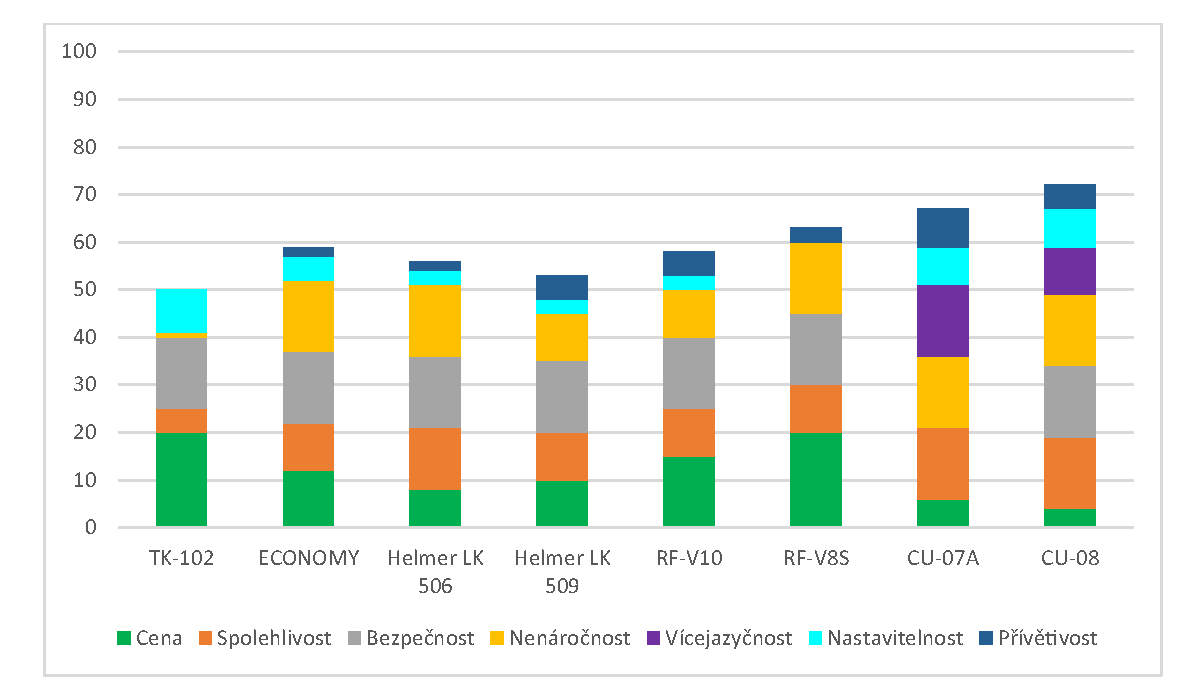
\includegraphics[width=\textwidth]{graphs/graf_bodoveHodnoceni.pdf}
\caption{Grafické znázornění bodového hodnocení dostupných modelů}
\label{image}
\end{center}
\end{figure}

% Koncept

\chapter{Koncept}
Při tvorbě konceptu jsem zaměřil na výběr obecných součástek, nespecifikuji tedy konkrétní výrobky, ale pouze jejich typ, díky čemuž není koncept svázán s určitým výrobkem a kusy lze nahradit jinými, které budou fungovat stejným způsobem. Dále jsem se zaměřil na způsob, jakým budou součástky propojeny, jak budou komunikovat a jak budou napájeny.

\section{Řídící jednotka}
Základem celého sledovacího zařízení je řídící jednotka, která ovládá veškeré dění, přijímá a zpracovává data, která následně vyhodnocuje. Na základě požadovaných vlastnostní jsem se rozhodl pro jednočipový počítač, dále jen mikrokontrolér, který je integrovaným obvodem, tedy v základní struktuře obsahuje procesor, operační paměť, paměť pro program, oscilátor, vstupní a výstupní rozhraní (porty). Mikrokontroléry se vyznačují velmi vysokou spolehlivostí, kompaktnostní a nízkou cenou, která je mým cílem. Často jsou využívány pro jednoúčelové aplikace řízení, nebo regulace.

\section{Komunikační rozhraní}
Komunikační rozhraní je zařízení, které poskytuje přístup do sítí GSM, GPS a popřípadě GPRS. Rozraní může obsahovat více komunikačních čipů, například jeden pro GPS, druhý pro GSM a tím umožní komunikaci v obou sítích zároveň. Nebo pomocí jednoho čipu, který kombinuje všechny sítě do jednoho zařízení, ale není možná komunikace ve více sítích zároveň, je tedy nutné mezi nimi přepínat. Komunikační rozraní musí poskytovat jednoduché příkazy, které umožní komunikovat přes zmíněné sítě, bez potřebné znalosti jejich interní struktury. Bude tedy možné pomocí jednoduchého příkazu odeslat zprávu SMS, nebo bude poskytovat data z GPS ve specifickém formátu, který bude možné zpracovat a vyhodnotit.

\section{Senzor pohybu}
Pro notifikaci změny pohybu a maximální úsporu elektrické energie a je nutné sledovací zařízení opatřit senzorem pohybu. Jedná se o čidlo, které zaznamenává změnu své vlastní polohy, nejedná tedy se o detektor pohybu, který zaznamenává pohyb okolí. Pro koncept je možné využít vibrační senzor, je levný (desítky korun), nepřesný (nelze nastavit přesnost) a používá jej většina dostupných modelů. Vibrační senzor má nulovou spotřebu, protože se jedná o drátek obmotný pružinkou, která se v případě pohybu dotkne drátku a uzavře se okruh. Dále je možné použít akcelerometr, který z porovnávaných modelů mají pouze modely od firmy Jablotron. Senzor je dražší (stovky korun) ale na druhou stranu je přesný (lze nastavit přesnost), spotřeba je u většiny modelů 10 mA. Možným řešením by byla detekce pohybu pomocí změny polohy GPS, nicméně spotřeba při připojení do sítě GPS se pohybuje kolem 200 mA, proto toto řešení označuji jako nevhodné, vzhledem k jeho nárokům na energii.

\section{Napájení}
Jako napájení může být použita autobaterie, nebo jakýkoliv jiný zdroj energie o minimálním napětí 12 V a minimálním výstupním proudem 1 A. Vstupní napětí 12 V je minimální potřebné napájecí napětí, které vyžaduje komunikační modul. Maximální velikost vstupního napětí bude dána použítým regulátorem napětí, který sníží vyšší napětí na požadované. Proudový odběr 1 A je maximální možný odběr, který bude zařízení schopno vyvinout. Při použití zdroje napájení s nížším maximálním proudem, než 1 A, může dojít k poklesu napětí, nebo nenávratnému poškození zdroje napájení (baterie), pokud je proud, které zařízení zrovna potřebuje vyšší, než proud který je zdroj napájení schopnen dodat. Poškozením je myšleno roztavení v některých případech i explozi (dle typu baterie). Mezi sledovací zařízení a zdroj napájení, bude umístěna vratná pojistka (PolySwitch), která ochrání sledovací zařízení před nadproudem či zkratem. 

\section{Blokové schéma}
Blokové schéma ukazuje propojení jednotlivých částí, do funkčního celku. Zdroj napájení je přes vratnou pojistku napojen na řídící jednotku, která dále rozděluje energii mezi další součástky, dle jejich potřeb (12 V, 5 V, 3 V). Řídící jednotka má na sebe napojen senzor pohybu, který indikuje změny pohybu a v případě změny, řídící jednotku probudí ze spánku. Na řídící jednotku je také napojeno komunikační rozhraní, které pouze vykonává příkazy řídící jednotky, popřípadě jí zasílá příchozí data. Dle typu komunikačního rozhraní je napojen na síť GPS, GSM, popřípadě GPRS.

\begin{figure}[H]
\begin{center}
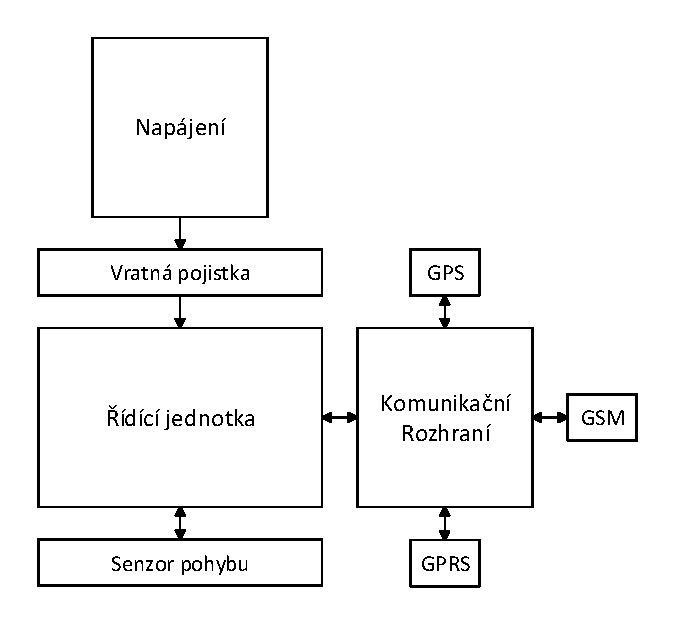
\includegraphics[width=\textwidth]{graphs/schema_blokove.pdf}
\caption{Blokové schéma zapojení}
\label{image}
\end{center}
\end{figure}

% Prototyp

\chapter{Prototyp}
Před tvorbou prototypu jsem se s vedoucí práce dohodl na využití hotových dílů, které poskládám dohromady a naprogramuji. Cílem této práce není vytvoření sledovacího zařízení, připraveného do sériové výroby, ale vytvoření prototypu na kterém ukáži zvolené hardwarové a softwarové řešení.

\section{Vývojová deska Arduino}
Jako řídící jednotku jsem si zvolil vývojovou desku Arduino UNO \cite{Arduino Schematic} od společnosti Arduino, která obsahuje čip ATmega328 \cite{Atmega datasheet}. Možnosti čipu i desky mnohonásobně přesahují požadavky na výkon i periferie, nicméně díky jednoduchému programování desky \cite{Pruvodce arduinem}, bude možný rychlý vývoj řídícího softwaru. V případě finální výroby navíc počítám s pouze jednodušší variantou čipu ATmega, takže finální kód by zůstal stejný. ATmega i jiná řešení jsou programována v jazyce C, tedy není problém s výměnou čipu za jiné řešení, pouze by bylo nutné upravit některé příkazy pro určitý čip. Čip řady ATmega používá jazyk C s knihovnou Wiring.

\begin{figure}[H]
\begin{center}
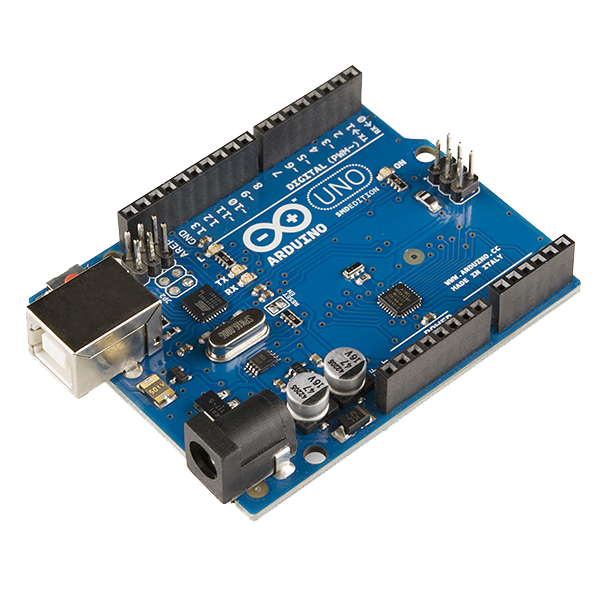
\includegraphics[width=0.5\textwidth]{images/arduino.png}
\caption{Vývojová deska Arduino UNO}
\label{image}
\end{center}
\end{figure}

\section{Komunikační modul GPS/GPRS/GSM}
Pro komunikaci jsem se rozhodl pro s arduinem kompatibilní desku, která zjednoduší propojení a umožní komunikačním modulem přímo rozšířit vývojovou desku Ardino. To nastane jednoduchým nasazením na desku, kdy jsou nožičky (piny) obou zařízení propojeny. Zvolil jsem řešení GPS/GPRS/GSM Module V3.0 \cite{ROBOT schematic} od firmy DFROBOT, které obsahuje možnost jednoduchého připojení všech možných periferií (mikrofon, reproduktor, sim karta, ...), čímž je skvělým modulem pro testování a vývoj. Hlavní částí je komunikační čip SIM908 \cite{SIMCOM HW}, který umí komunikovat přes GPS, GSM i GPRS a navíc je jednoduše ovladatený \cite{SIMCOM SW}. Čipy řady SIM900 jsou využívány ve všech nalezených sledovacích zařízeních, jedná se o jedno z mála dostupných řešení, které je levné a v případě budoucí výroby předpokládám jeho použití, proto bude software postaven na komunikaci s tímto čipem.

\section{Akcelerometr}
Not supported yet.

%Softwarový návrh

\chapter{Softwarový návrh}
Not supported yet.

\section{Prostředí Arduino}
Not supported yet.

\section{Knihovna Wiring}
Not supported yet.

\section{Diagram tříd}
Not supported yet.

\section{Výpočet polohy z dat GPS}
Not supported yet.

% Závěr

\chapter{Závěr}
Not supported yet.

\begin{thebibliography}{References}
\bibitem{LaTeX}SATRAPA, Pavel. LaTeX pro pragmatiky [online]. 2011, 87 s. [cit. 2016-05-07]. Dostupné z: http://www.nti.tul.cz/~satrapa/docs/latex/latex-pro-pragmatiky.pdf
\bibitem{LaTeX}SATRAPA, Pavel. Stručný přehled příkazů LaTeXu [online]. 2011, 2 s. [cit. 2016-05-07]. Dostupné z: http://www.nti.tul.cz/~satrapa/docs/latex/latex-prehled.pdf
\bibitem{SIFT}SIRF TECHNOLOGY, INC. NMEA Reference Manual [online]. 2.1. San Jose., 2007, 27 s. [cit. 2016-05-07]. Dostupné z: https://www.sparkfun.com/datasheets/GPS/NMEA\%20Reference\% 20Manual-Rev2.1-Dec07.pdf
\bibitem{CSR}CSR PLC. NMEA Reference Guide [online]. 2. Cambridge: CSR plc, 2011, 50 s. [cit. 2016-05-07]. Dostupné z: http://www.inventeksys.com/wp-content/uploads/2012/05/NMEA-Reference-Manual-CS-129435-MA-2.pdf
\bibitem{SIMCOM HW}SIMCOM WIRELESS SOLUTIONS. SIM908 Hardware Design [online]. 2. Jinzhong, 2012, 53 s. [cit. 2016-05-07]. Dostupné z: http://www.niplesoft.net/blog/wp-content/uploads/2016/02/SIM908-Hardware-Design-V2.00-1.pdf
\bibitem{SIMCOM SW}SIMCOM WIRELESS SOLUTIONS. SIM908 AT Command Manual [online]. Jinzhong, 2011, 249 s. [cit. 2016-05-07]. Dostupné z: http://www.dfrobot.com/image/data/TEL0051/3.0/ SIM908\_AT\%20Command\%20Manua\_V1.01.pdf
\bibitem{ROBOT schematic}DFROBOT. GSM+GPRS+GPS V3.0 schematic [online]. Shanghai, 2013, 1 s. [cit. 2016-05-07]. Dostupné z: http://www.dfrobot.com/image/data/TEL0051/GSM+GPRS+GPS \%20SIM908\%20V3.0.pdf
\bibitem{ROBOT SW}GPS/GPRS/GSM Module V3.0 (SKU:TEL0051). DFRobot Wiki [online]. [cit. 2016-05-07]. Dostupné z: http://www.dfrobot.com/wiki/index.php/GPS/GPRS/GSM\_Module \_V3.0\_(SKU:TEL0051)
\bibitem{Arduino Schematic}ARDUINO LLC. Arduino Schematic [online]. 1 s. [cit. 2016-05-07]. Dostupné z: https://www.arduino.cc/en/uploads/Main/Arduino\_Uno\_Rev3-schematic.pdf
\bibitem{Pruvodce arduinem}VODA, Zbyšek. Průvodce světem Arduina [online]. Vydání první. Bučovice: Martin Stříž, 2015 [cit. 2016-05-07]. ISBN 978-80-87106-90-7.
\bibitem{Atmega datasheet}ATMEL CORPORATION. ATmega48A/PA/88A/PA/168A/PA/328/P Datasheet [online]. 2015, 660 s. [cit. 2016-05-07]. Dostupné z: http://www.atmel.com/images/Atmel-8271-8-bit-AVR-Microcontroller-ATmega48A-48PA-88A-88PA-168A-168PA-328-328P\_datasheet\_Complete.pdf


\end{thebibliography}

\end{document}